\chapter{Dise\~no de la Soluci\'on}\label{ch:solution}

Los capítulos anteriores presentan la problemática y detallan la arquitectura, una vez hecho esto podemos definir el camino a tomar para la solución, nuestra solución constará de 3 partes:

\begin{itemize}
\item Simulador
\item Sistema Linux
\item Diseño de hardware
\end{itemize}

En las siguientes secciones se detallan éstas partes de la solución.

\section{Simulador}

El simulador se desarrollará para reducir el tiempo al trabajar con microcontroladores \ac{ARM} y simular los dispositivos que se desee, a continuación presentamos un breve análisis de requerimientos para posteriormente pasar a la arquitectura del simulador.

\subsection{Requerimientos funcionales}

\begin{itemize}
\item Simular conjunto de instrucciones \ac{ARM}.
\item Fácil simulación de componentes.
\item Fácil integración de componentes con simulador ARM.
\item Uso sencillo para el usuario final, facilidad de simulación y programación del dispositivo.
\end{itemize}

\subsection{Requerimientos no funcionales}

\begin{itemize}
\item Ejecución solamente en ambiente UNIX.
\item Simula conjunto de instrucciones ARM, no Thumb ni Jazelle.
\item Programación en C y ensamblador únicamente.
\end{itemize}

De acuerdo a los requerimientos funcionales y no funcionales podemos describir los casos de uso con el diagrama de la figura \ref{Flo:uso}
Para dar al usuario estas capacidades y al mismo tiempo permitir flexibilidad en el simulador se ha diseñado una arquitectura que se muestra en la figura \ref{Flo:implementacion_memoria}, se propone implementar un buffer para la memoria de cada dispositivo, el microprocesador ve una lista de nodos, cada nodo describe cual es la dirección de inicio y su tamaño.	

\begin{figure}
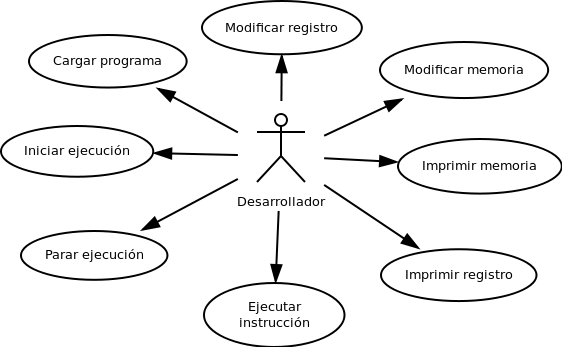
\includegraphics[scale=0.5]{img/uso}\caption{Diagrama de casos de uso}
\label{Flo:uso}
\end{figure}

\begin{figure}
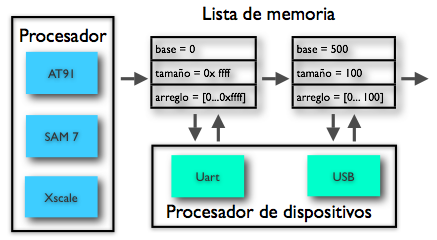
\includegraphics[scale=0.7]{img/implementacion_memoria}\caption{Implementación de modelo de memoria}
\label{Flo:implementacion_memoria}
\end{figure}

En la figura \ref{figura_arq} se detalla la arquitectura propuesta para el simulador.
Como se puede observar hay una interfaz del simulador con cada uno de los componentes, la interfaz es común para los componentes, en el caso de los microcontroladores se usan los registros, y en el caso de los componentes la memoria compartida del microprocesador.
Se han desarrollado bibliotecas que permiten la modelación de dispositivos externos con código sencillo y con ellas se han llevado a cabo pequeños experimentos donde se realizan las simulaciones de pequeños componentes de \ac{ARM}.

\begin{figure}
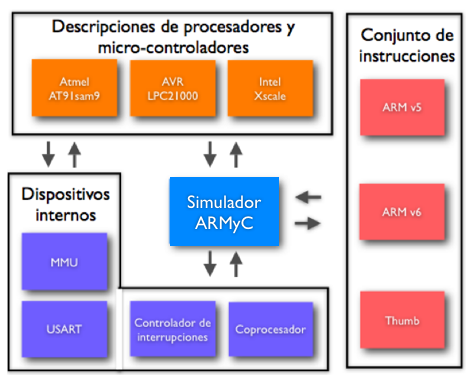
\includegraphics[scale=0.7]{img/figura_arq}\caption{Modelo de la arquitectura del simulador}
\label{Flo:figura_arq}
\end{figure}

\section{Sistema Linux}

Una sección importante de este trabajo se refiere a la facilidad de portar el ambiente a un sistema físico, Linux provee de esa característica de una manera sencilla.

Debido a que Linux ya se ha portado a la arquitectura ARM, se tiene la confianza de que es una solución probada, y provee de la funcionalidad necesaria para portar a nuevas tarjetas.

\section{Dise\~no de hardware}

Este trabajo busca facilitar el diseño de dispositivos basados en la tecnología ARM, y para ello se buscó un caso de estudio de una tarjeta real.

Se llevó a cabo el diseño de esta tarjeta y se implementó una parte considerable de los dispositivos diseñados en la misma.

Para ello se tuvo que llevar a cabo un diseño del diagrama físico, que cumpliera con las siguientes características:

\begin{itemize}
\item Sencillez para extenderlo.
\item Generar la documentación para entender el proyecto base.
\item Proveer tanto diseño esquemático como PCB.
\end{itemize}

\section{Funciones}

Para cumplir con los objetivos de este proyecto es deseable que el
diseño del sistema pueda ser utilizado para construir posteriormente
dispositivos m\'{o}viles, que adem\'{a}s de manejar video en dos dimensiones,
pueda utilizar una gran variedad de dispositivos externos tales como: 
\begin{itemize}
\item Internet inal\'{a}mbrico por medio de WiFi.
\item Video en una pantalla LCD.
\item Dispositivos de Entrada y Salida.
\end{itemize}
Para ser usada como plataforma de desarrollo es necesario ser capaces
de subir c\'{o}digo a la tarjeta de una manera sencilla los nuevos
programas y cambios que desarrollemos. 

Otro punto importante a tomar en cuenta es la salida de video, para
ello se deben de poder guardar imágenes en una memoria de alta capacidad
y poderlas trabajar en una memoria de mejor velocidad. 

Es por ello que se han definido las siguientes capacidades importantes
de la tarjeta:
\begin{itemize}
\item Reguladores de Voltaje a 3.3 volts.
\item Interfaz USB para fácil acceso a la computadora.
\item Interfaz con dispositivos de almacenamiento externos.
\item Interfaz para depurar y programación c\'{ó}digo.
\item Capacidad de conectar dispositivos de memoria externa. 
\end{itemize}
Los dispositivos que se han seleccionado para cumplir con esta especificaci\'{o}n
se detallarán a continuación.\pagebreak{}
